\chapter{User Interface Design \& Implementation}

\section{Updated Pages}

\subsection{Home Page}
\begin{figure}[H]
\centering
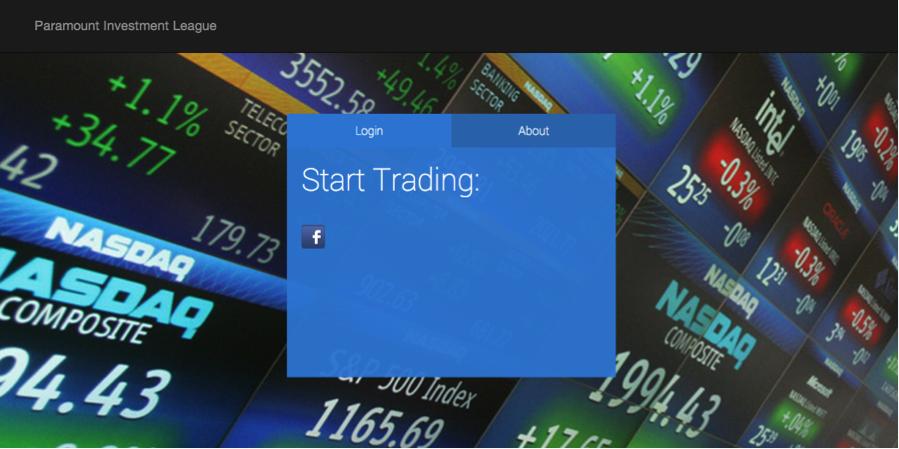
\includegraphics[width=5.5in]{./img/ui/1.png}
\caption{This graphic illustrates the relationships between the core actors of our platform.}
\end{figure}

\subsection{Home Page}
\begin{figure}[H]
\centering
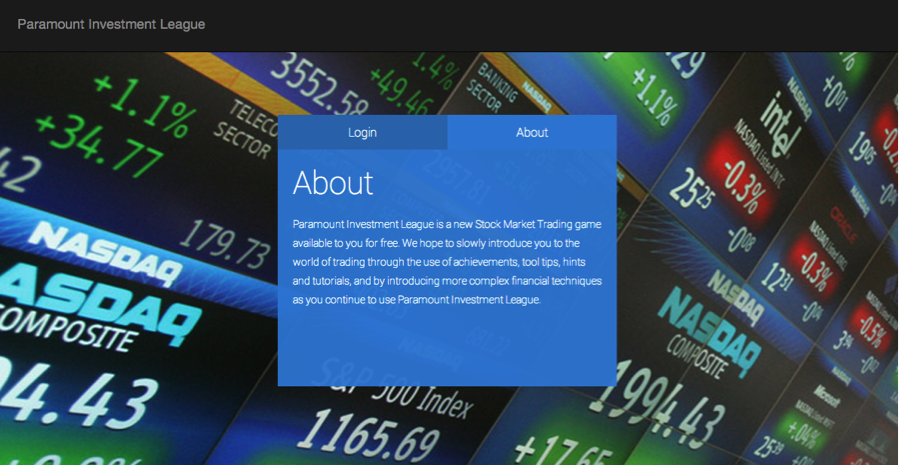
\includegraphics[width=5.5in]{./img/ui/2.png}
\caption{This graphic illustrates the relationships between the core actors of our platform.}
\end{figure}

\subsection{Home Page}
\begin{figure}[H]
\centering
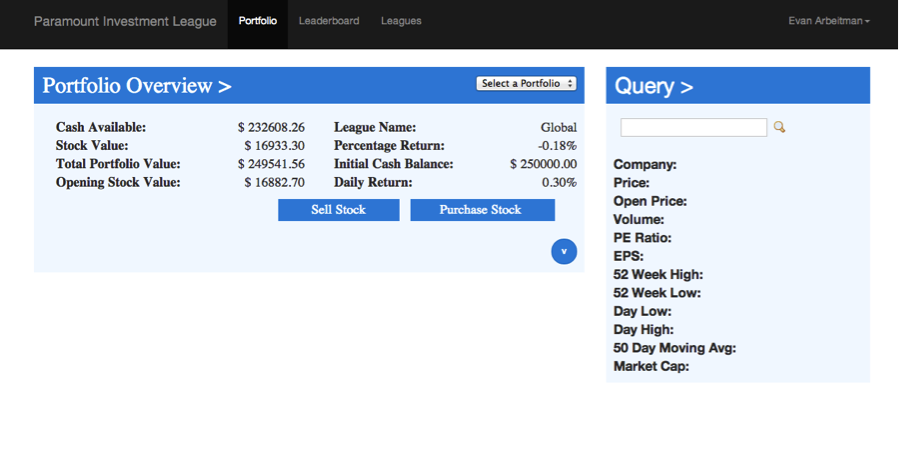
\includegraphics[width=5.5in]{./img/ui/3.png}
\caption{This graphic illustrates the relationships between the core actors of our platform.}
\end{figure}

\subsection{Home Page}
\begin{figure}[H]
\centering
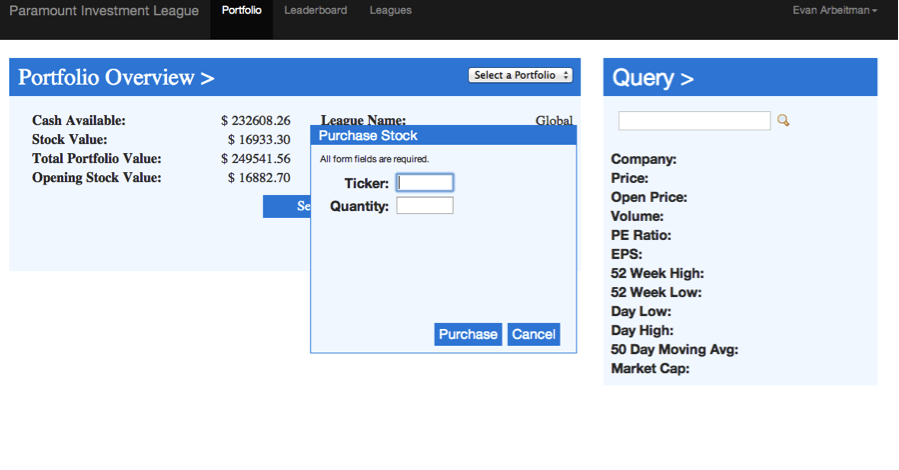
\includegraphics[width=5.5in]{./img/ui/4.png}
\caption{This graphic illustrates the relationships between the core actors of our platform.}
\end{figure}

\subsection{Home Page}
\begin{figure}[H]
\centering
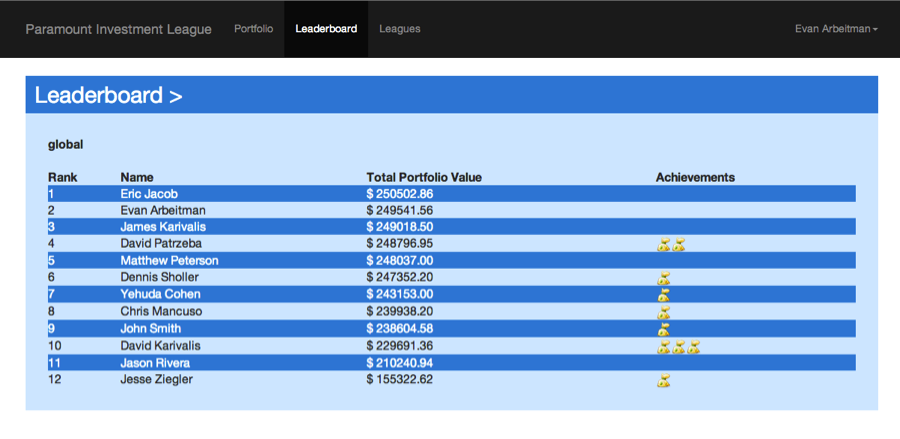
\includegraphics[width=5.5in]{./img/ui/5.png}
\caption{This graphic illustrates the relationships between the core actors of our platform.}
\end{figure}

\subsection{Home Page}
\begin{figure}[H]
\centering
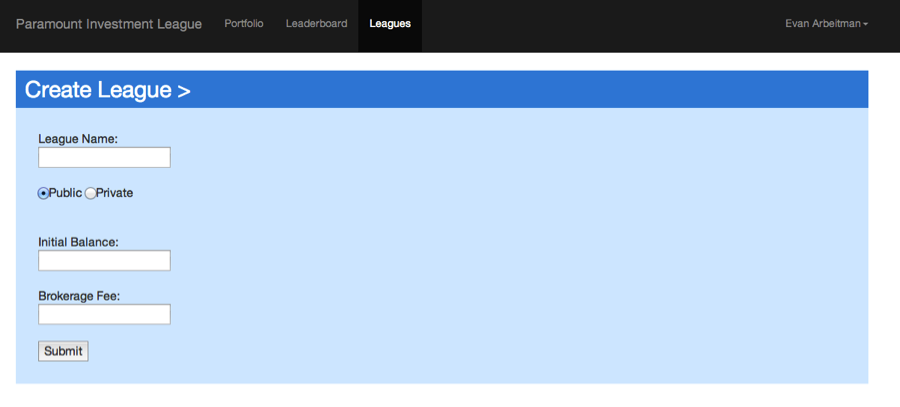
\includegraphics[width=5.5in]{./img/ui/6.png}
\caption{This graphic illustrates the relationships between the core actors of our platform.}
\end{figure}

\subsection{Home Page}
\begin{figure}[H]
\centering
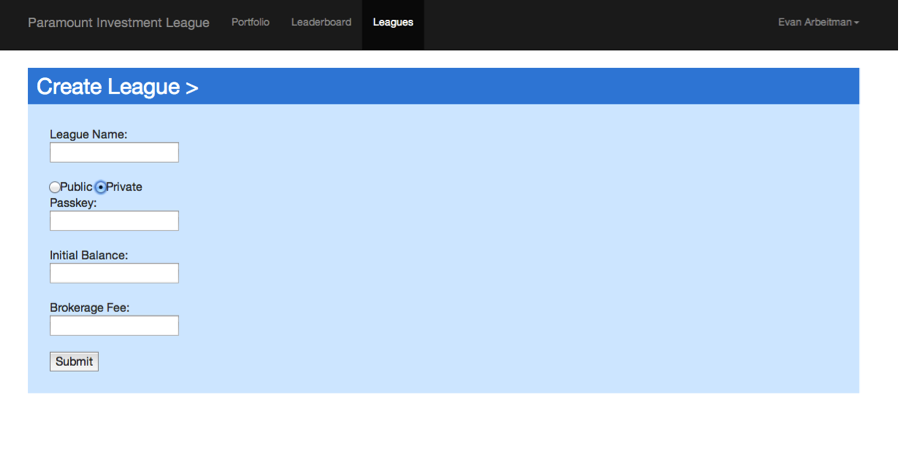
\includegraphics[width=5.5in]{./img/ui/7.png}
\caption{This graphic illustrates the relationships between the core actors of our platform.}
\end{figure}

\subsection{Home Page}
\begin{figure}[H]
\centering
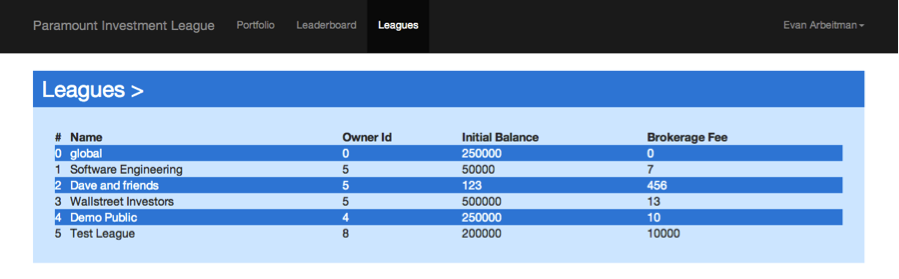
\includegraphics[width=5.5in]{./img/ui/8.png}
\caption{This graphic illustrates the relationships between the core actors of our platform.}
\end{figure}

\subsection{Home Page}
\begin{figure}[H]
\centering
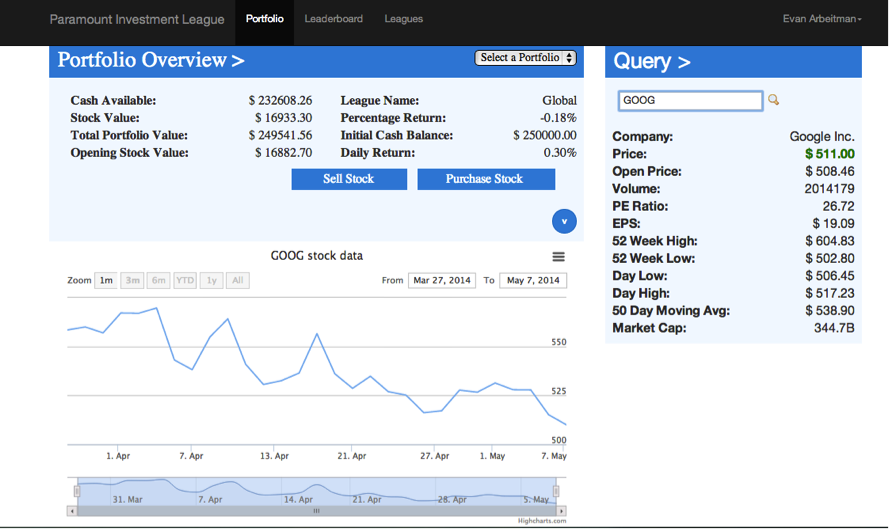
\includegraphics[width=5.5in]{./img/ui/9.png}
\caption{This graphic illustrates the relationships between the core actors of our platform.}
\end{figure}


\section{Efficiency of the Views}

One thing that we need to concentrate on is ensuring that the website is fast
for all users no matter what kind of device or connection the end user is using.
For this reason, you will see a logical breakdown of the website which will
allow us to cache elements of the site on the client side that generally won't
change.  We do this be separating the header, ticker, and the content of a given
page.  Since the header and ticker are the same across the entire site, they
only need be loaded on the client a single time, and can be cached on the client
side for the duration of the visit or longer.\\

The content of each individual page is dynamic, but by harnessing technologies
like AJAX\cite{wiki:ajax} and Comet\cite{wiki:comt}, we are able to indicate to
the user that the page
is always reacting to their inputs without reloading the page.  This again
allows us to cache the resulting page on the client side, an perform updates
as needed with minimal delay.\\

To further assist with reducing the load on clients, we will be using
HTML\cite{wiki:html} and CSS\cite{wiki:css} to present our User Interface
relying very minimally on pictures.  Any picture that is displayed will be
resized to the maximum allowed size and contained in an appropriate web format.\\

Finally, as discussed much throughout these reports, our goal is to be able to
present our application across as many device as possible, including mobile,
tablet, and desktop.  We accomplish this by relying on the Twitter
Bootstrap\cite{wiki:boot} CSS framework to help facilitate creating a responsive
website.\\

Of course this all comes with a trade off, that is we won't support older
browsers incapable of displaying and parsing HTML5/CSS3/JS or aren't web
compliant with modern web standards.  This should have minimal impact however,
since most devices and users have a modern web browser, and those that don't
generally don't fall into our target audience.\\

\section{Home Page}

